\documentclass[12pt]{report}
\usepackage[print,nopanel]{pdfscreen}
\begin{print}
\usepackage{lipsum}
\usepackage{titletoc}
\usepackage{lastpage}
\usepackage{macro/macro}
\usepackage{float}
\usepackage{wrapfig}
\usepackage{fancyhdr}
\usepackage{verbatim}
\usepackage{scrextend}

\usepackage[Glenn]{fncychap}
\lhead{\large\bfseries\   }
\usepackage[left=3.5cm, right=1.25cm, top=2.5cm, bottom=1.25cm]{geometry}
\pagestyle{fancy}
\end{print}
\margins{.5cm}{.5cm}{.5cm}{.5cm}
\begin{screen}

\renewcommand{\encodingdefault}{T1}
\usepackage{setspace}
\linespread{1.5}
\renewcommand{\rmdefault}{ptm}
\end{screen}
\screensize{8cm}{9cm}
\overlay{overlay8.pdf}
\usepackage{graphicx}

\usepackage{listings}

\begin{document}
\newcommand{\centertext}[1]{\begin{center}\textbf{#1}\end{center}}
\newcommand{\student}{\vskip 2.5cm}
\newcommand{\supervisor}{\vskip 2cm}
\newcommand{\stamp}{\vskip 2.5cm}
\newcommand{\HRule}{\rule{\linewidth}{0.5mm}}
\newcommand{\projecttitle}{\Huge {Pdf Club }\vskip 0.1in}
\newcommand{\tab}[1]{\hspace{.4\textwidth}\rlap{#1}}
\newcommand{\itab}[1]{\hspace{.05\textwidth}\rlap{#1}}
\newcommand{\logo}[1]{\includegraphics[scale=0.7]{#1}}
\newcommand{\submitted}{


\vskip 0.2in
\vskip 0.7cm
\large\bf{\bf REPORT}\\
\vskip 0.5cm
\textnormal{
SUBMITTED IN PARTIAL FULFILLMENT OF THE REQUIREMENT FOR
\\Six Month Industrial Training
}
\vskip 0.2cm
\textnormal{at}
\vskip 0.2cm

\large\bf{\bf Auribises Technologies, Ludhiana
\\(from June 5,2017 to December 5,2017)
}



\vskip 1.7cm
\textnormal{Submitted By \vspace{5pt} \\ Navjot Singh (1411289) \\ Manpreet Singh (1411281) 
\\Deepak Pruthi(1411248)}

\vskip 0.5cm
%\image{0.7}{images/gne.png}{}
\logo{images/gne.png}
\vskip 3.0cm


%\image{0.7}{images/gne.png}{}
%\logo{images/gne.png}
%\vskip 3.0cm

\HRule \\[0.4cm]

\textnormal \bf{ \bf Information Technology Department} 
\large \bf{ \bf \\GURU NANAK DEV ENGINEERING COLLEGE } 
\large { \\LUDHIANA, INDIA }
 }


\newcommand{\pagetitle}{\begin{center}
\projecttitle
\Large\textbf{}\\
\submitted
\vskip 1cm

\end{center}}
\newcommand{\openoffice}{\textbf{OpenOffice}}
\newcommand{\frontmatter}[1]{\begin{Large} \textbf{#1} \end{Large}}
\newcommand{\ppttitle}{\begin{center}
\end{center}}

\begin{screen}
\ppttitle
\end{screen}
\footskip 0.7cm
\thispagestyle{empty} 
\pagetitle
\newpage
\pagenumbering{Roman}
\cfoot{\thepage}
%
\begin{figure}[ht]
\centering

\includegraphics[scale=0.5]{images/cer.png}
\end{figure}
\newpage
\begin{Large}
\centertext{Acknowledgement}
\end{Large}
\vskip 0.1in I am  highly grateful to ​
Dr. M.S. Saini Director, Guru Nanak Dev Engineering  
College, Ludhiana for providing this opportunity to carry out minor project at Guru Nanak  
Dev Engineering College. The constant guidance and encouragement received from ​
ER. Inderjeet Singh, Assistant Professor, Department of IT has been of great help in carrying out the project work and is acknowledged with reverential thanks.

I would like to express a deep sense of gratitude and thanks profusely to DR. K.S. Mann, Guru Nanak Dev Engineering College. Without his wise counsel and able guidance, it would have been impossible to complete the report in this manner. The author expresses gratitude to other faculty members of IT department of GNDEC for their intellectual support throughout the course of this work.

Last, but not the least I wish to thank my parents and friends who directly or indirectly have given me moral support and their relentless advice throughout the completion of this project work. 

\vskip 0.4in
\noindent \textbf{Gurnoor Singh}


\newpage
\begin{Large}
\centertext{Abstract}
\end{Large}
\vskip 0.1in Modern life offers a plethora of options of services and goods for consumers. As a 
result, people’s expenses have gone up dramatically, e.g., compared to a decade ago, and the 
cost of living has been increasing day by day. Thus it becomes essential to keep a check on expenses in order to live a good life with a proper budget set up.  \\

\noindent The Android OS smartphones is one of the top-selling  in the world ,it is apparent that people have been using smartphones as an organizational tool. .\\

\noindent In this application, User can upload and download E-books based upon preference.User can also enter
Description, date , name  and other optional attributes ( Adding categories  to the E-books). With this entered information, the user is able to see the name, file size, description, upload date and many other details of ebook 


\newpage
\tableofcontents
\newpage
\listoffigures
\newpage

\pagenumbering{arabic}
\cfoot{\thepage}

\newpage
\chapter{Introduction}
\section{Introduction to Organization}

Forget about not remembering where you spent your money! Keep track of your expenses and get
a lot of statistics to know in what you spend more and you can evaluate where you can cut some expenses! Take advantage of this tool that will help you to manage your money and be informed
all the time. You can also configure to get notifications when you have to make some payments
every month so you dont forget! This Application is made for any user who wants or wish to keep a better track of their expenses in order to keep them in a same place.
\section{Introduction To Project} 
With the launch and increase in sales of smartphones over the last few years, people are using mobile applications to get their work done, which makes their lives easier. Mobile applications comprise various different categories such as Entertainment, Sports, Lifestyle, Education, Games, Food and Drink, Health and Fitness, Finance, etc. This Expense Tracker application falls in the Finance Category and serves the important purpose of managing finances which is a very important part of one’s life.  The software product went through the design, development, and the testing phase as a part of the Software Development Lifecycle. 

The application’s interface is designed using custom art elements, the functionality is implemented using Android SDK, and the phase of testing the product was accomplished successfully. The application is not much user intensive but just comprises of having them enter the expense amount, date, category, merchant and other optional attributes (taking picture of the receipts, entering notes about the expense, adding subcategories to the categories). With this entered information, the user is able to see the expense details daily, weekly, monthly, and yearly in figures, graphs. All these topics have been explained in detail in their respective chapters

\section{Project Category(Internet based, Application or System Development, Research based ,Industry Automation, Network or System Administration)}

\section{Objectives}

\begin{itemize}
	\item Implement the various concepts of Android programming together within an application that becomes helpful for intended users.
	\item Developing an Android based money management system having user friendly interface.
\end{itemize}
 

\section{Problem Formulation}
yo

\section{Identification/Reorganization of Need}

\section{Existing System}

\section{Proposed System}

\section{Unique Features of the System}




\newpage
%\chapter{\LaTeX}
%

\LaTeX, I have used this tool for preparing my six weeks training report and i found it excellent. So this time again i decided to use it for my report.
\LaTeX{} (pronounced /ˈleɪtɛk/, /ˈleɪtɛx/, /ˈlɑːtɛx/, or /ˈlɑːtɛk/) is a 
document markup language and document preparation system for the \TeX{} 
typesetting  program. Within the typesetting system, its name is styled 
as \LaTeX.

\image{0.9}{images/donald.png}{Donald Knuth, Inventor Of \TeX{} 
typesetting system}

\noindent Within the typesetting system, its name is styled as \LaTeX. The term 
\LaTeX{} refers only to the language in which documents are written, 
not to the editor used to write those documents. In order to create a 
document in \LaTeX, a .tex file must be created using some form of text 
editor. While most text editors can be used to create a \LaTeX{} document, 
a number of editors have been created specifically for working with \LaTeX.\\

\noindent \LaTeX{} is most widely used by mathematicians, scientists, 
engineers, philosophers, linguists, economists and other scholars in 
academia. As a primary or intermediate format, e.g., translating DocBook 
and other XML-based formats to PDF, \LaTeX{} is used because of the 
high quality of typesetting achievable by \TeX. The typesetting system 
offers programmable desktop publishing features and extensive facilities 
for automating most aspects of typesetting and desktop publishing, 
including numbering and cross-referencing, tables and figures, 
page layout and bibliographies.\\

\noindent \LaTeX{} is intended to provide a high-level language that
accesses the power of \TeX. \LaTeX{} essentially comprises a
collection of \TeX{} macros and a program to process \LaTeX documents. 
Because the \TeX{} formatting commands are very low-level, it is usually 
much simpler for end-users to use \LaTeX{}.


\section{Typesetting}
\LaTeX{} is based on the idea that authors should be able to focus on 
the content of what they are writing without being distracted by its 
visual presentation. In preparing a \LaTeX{} document, the author 
specifies the logical structure using familiar concepts such as 
chapter, section, table, figure, etc., and lets the \LaTeX{} system 
worry about the presentation of these structures. It therefore 
encourages the separation of layout from content while still allowing 
manual typesetting adjustments where needed. 

\begin{verbatim}
\documentclass[12pt]{article}
\usepackage{amsmath}
\title{\LaTeX}
\date{}
\begin{document}
  \maketitle 
  \LaTeX{} is a document preparation system 
  for the \TeX{} typesetting program.
   \par 
   $E=mc^2$
\end{document}
\end{verbatim}

\subsection{Installing \LaTeX{} on System}
Installation of \LaTeX{} on personal system is quite easy. As i have used \LaTeX{} on Ubuntu 14.04 so i am discussing the installation steps for Ubuntu 14.04 here:\\
\begin{itemize}
\item Go to terminal and type\\
\textit{sudo apt-get install texlive-full}
\item Your Latex will be installed on your system and you can check for manual page by typing.\\
\textit{man latex}
in terminal which gives manual for latex command.
\item To do very next step now one should stick this to mind that the document which one is going to produce is written in any type of editor whether it may be your most common usable editor Gedit or you can use vim by installing first vim into your system using command.\\
\textit{sudo apt-get install vim}
\item After you have written your document it is to be embedded with some set of commands that Latex uses so as to give a structure to your document. Note that whenever you wish your document to be looked into some other style just change these set of commands.
\item When you have done all these things save your piece of code with .tex format say test.tex. Go to terminal and type\\
\textit{latex path of the file test.tex Or pdflatex path of the file test.tex\\ eg: pdflatex test.tex}
for producing pdf file simultaneously.\\
After compiling it type command\\\\
\textit{evince filename.pdf\\ eg: evince test.pdf}\\
To see output pdf file. 
\end{itemize}

\subsection{Graphical Editors for \LaTeX{}}
\LaTeX{} is not restricted to command line only there are so many graphical based editors available to be used. These GUi based editors provide an easy interface to user so as to do typesetting in an efficient manner. Some of them are listed below:
\begin{itemize}
\item Tex Maker
\item LED 
\end{itemize}
And many more but the preferred method to produce \LaTeX{} document is through console mode only.

%\chapter{Literature Review}
%

\chapter{Requirement Analysis and System Specification}
\section{Feasibility Study (Technical,Economical,Operational)}
Feasibility study is made to see if the project on completion will serve the purpose of the organization for the amount of work, effort and the time that spend on it. Feasibility study lets the developer foresee the future of the project and the usefulness. A feasibility study of a system proposal is according to its workability, which is the impact on the organization, ability to meet their user needs and effective use of resources. Carrying out a feasibility study involves information assessment, information collection and report writing. The information assessment phase identifies the information that is required to answer the three questions set out above. Once the information has been identified, you should question information sources to discover the answers to these questions Thus when a new application is proposed it normally goes through a feasibility study before it is approved for development.

A feasibility study is designed to provide an overview of the primary issues related to a business idea.  The purpose is to identify any “make or break” issues that would prevent your business from being successful in the marketplace. In other words, a feasibility study determines whether the business idea makes sense. A thorough feasibility analysis provides a lot of information necessary for the business plan.  For example, a good market analysis is necessary in order to determine the project’s feasibility.  This information provides the basis for the market section of the business plan.

The document provide the feasibility of the project that is being designed and lists various areas that were considered very carefully during the feasibility study of this project such as Technical, Economic and Operational feasibilities. Feasibility is defined as the practical extent to which a project can be performed successfully. To evaluate feasibility, a feasibility study is performed, which determines whether the solution considered to accomplish the requirements is practical and workable in the software. Information such as resource availability, cost estimation for software development, benefits of the software to the organization after it is developed and cost to be incurred on its maintenance are considered during the feasibility study. The objective of the feasibility study is to establish the reasons for developing the software that is acceptable to users, adaptable to change and conformable to established standards.

Objectives of feasibility study are listed below.
\begin{itemize}
	\item To analyze whether the software will meet organizational requirements
	\item To determine whether the software can be implemented using the current technology and within the specified budget and schedule
	\item To determine whether the software can be integrated with other existing software.
\end{itemize}

\subsection{Types of Feasibility}
Various types of feasibility that are commonly considered include technical feasibility, operational feasibility, and economic feasibility.

\subsubsection{Technical Feasibility}
Technical feasibility is one of the first studies that must be conducted after the project has been identified. In large engineering projects consulting agencies that have large staffs of engineers and technicians conduct technical studies dealing with the projects. In individual agricultural projects financed by local agricultural credit corporations, the technical staff composed of specialized agricultural engineers, irrigation and construction engineers, and other technicians are responsible for conducting such feasibility studies. The technical feasibility assessment is focused on gaining an understanding of the present technical resources of the organization and their applicability to the expected needs of the proposed system. It is an evaluation of the hardware and software and how it meets the need of the proposed system. This assessment is based on an outline design of system requirements, to determine whether the company has the technical expertise to handle completion of the project. When writing a feasibility report, the following should be taken to consideration:
\begin{itemize}
	\item A brief description of the business to assess more possible factors which could affect the study
	\item The part of the business being examined
	\item The human and economic factor
	\item The possible solutions to the problem
\end{itemize}

The system must be evaluated from the technical point of view first. The assessment of this feasibility must be based on an outline design of the system requirement in the terms of input, output, programs and procedures. Having identified an outline system, the investigation must go on to suggest the type of equipment, required method developing the system, of running the system once it has been designed. Technical feasibility assesses the current resources (such as hardware and software) and technology, which are required to accomplish user requirements in the software within the allocated time and budget. For this, the software development team ascertains whether the current resources and technology can be upgraded or added in the software to accomplish specified user requirements. Technical feasibility also performs the following tasks.

\begin{itemize}
	\item Analyzes the technical skills and capabilities of the software development team members
	\item Determines whether the relevant technology is stable and established
	\item Ascertains that the technology chosen for software development has a large number of users so that they can be consulted when problems arise or improvements are required.
\end{itemize}

Technical issues raised during the investigation are:
\begin{itemize}
	\item Does the existing technology sufficient for the suggested one?
	\item Can the system expand if developed?
\end{itemize}

The project should be developed such that the necessary functions and performance are achieved within the constraints. The project is developed within latest technology. Through the technology may become obsolete after some period of time, due to the fact that never version of same software supports older versions, the system may still be used. So there are minimal constraints involved with this project. The system has been developed using Java the project is technically feasible for development.

\subsubsection{Economic Feasibility}
The purpose of the economic feasibility assessment is to determine the positive economic benefits to the organization that the proposed system will provide. It includes quantification and identification of all the benefits expected. This assessment typically involves a cost/ benefits analysis.

Economic feasibility is the cost and logistical outlook for a business project or endeavor. Prior to embarking on a new venture, most businesses conduct an economic feasibility study, which is a study that analyzes data to determine whether the cost of the prospective new venture will ultimately be profitable to the company. Economic feasibility is sometimes determined within an organization, while other times companies hire an external company that specializes in conducting economic feasibility studies for them.

The purpose of business in a capitalist society is to turn a profit, or to earn positive income. While some ideas seem excellent when they are first presented, they are not always economically feasible. That is, that they are not always profitable or even possible within a company's budget. Since companies often determine their budget's several months in advance, it is necessary to know how much of the budget needs to be set aside for future projects. Economic feasibility helps companies determine what that dollar amount is before a project is ultimately approved. This allows companies to carefully manage their money to insure the most profitable projects are undertaken. Economic feasibility also helps companies determine whether or not revisions to a project that at first seems unfeasible will make it feasible.

The developing system must be justified by cost and benefit. Criteria to ensure that effort is concentrated on project, which will give best, return at the earliest. One of the factors, which affect the development of a new system, is the cost it would require. Economic feasibility determines whether the required software is capable of generating financial gains for an organization. It involves the cost incurred on the software development team, estimated cost of hardware and software, cost of performing feasibility study, and so on. For this, it is essential to consider expenses made on purchases (such as hardware purchase) and activities required to carry out software development. In addition, it is necessary to consider the benefits that can be achieved by developing the software. Software is said to be economically feasible if it focuses on the issues listed below.
\begin{itemize}
	\item Cost incurred on software development to produce long-term gains for an organization.
	\item Cost required to conduct full software investigation (such as requirements elicitation and requirements analysis).
	\item Cost of hardware, software, development team, and training.
\end{itemize}

The following are some of the important financial questions asked during preliminary investigation:
\begin{itemize}
	\item The costs conduct a full system investigation.
	\item The cost of the hardware and software.
	\item The benefits in the form of reduced costs or fewer costly errors.
\end{itemize}

Since the system is developed as part of project work, there is no manual cost to spend for the proposed system. Also all the resources are already available, it give an indication of the system is economically possible for development.

\subsubsection{Operational Feasibility}
Behavioral feasibility assesses the extent to which the required software performs a series of steps to solve business problems and user requirements. It is a measure of how well the solution of problems or a specific alternative solution will work in the organization. It is also measure of how people feel about the system. If the system is not easy to operate, than operational process would be difficult. The operator of the system should be given proper training. The system should be made such that the user can interface the system without any problem.

Operational feasibility is a measure of how well a proposed system solves the problems, and takes advantage of the opportunities identified during scope definition and how it satisfies the requirements identified in the requirements analysis phase of system development. The operational feasibility assessment focuses on the degree to which the proposed development projects fits in with the existing business environment and objectives with regard to development schedule, delivery date, corporate culture, and existing business processes.

To ensure success, desired operational outcomes must be imparted during design and development. These include such design-dependent parameters such as reliability, maintainability, supportability, usability, producibility, disposability, sustainability, affordability and others. These parameters are required to be considered at the early stages of design if desired operational behaviors are to be realized. A system design and development requires appropriate and timely application of engineering and management efforts to meet the previously mentioned parameters. A system may serve its intended purpose most effectively when its technical and operating characteristics are engineered into the design. Therefore, operational feasibility is a critical aspect of systems engineering that needs to be an integral part of the early design phasesThis feasibility is dependent on human resources (software development team) and involves visualizing whether the software will operate after it is developed and be operative once it is installed. Operational feasibility also performs the following tasks.

\begin{itemize}
	\item Determines whether the problems anticipated in user requirements are of high priority.
	\item Determines whether the solution suggested by the software development team is acceptable.
	\item Analyzes whether users will adapt to a new software.
	\item Determines whether the organization is satisfied by the alternative solutions proposed by the software development team.
\end{itemize}

This includes the following questions:
\begin{itemize}
	\item Is there sufficient support for the users?
	\item Will the proposed system cause harm?
	\item The project would be beneficial because it satisfies the objectives when developed and installed. All behavioral aspects are considered carefully and conclude that the project is behaviorally feasible.
\end{itemize}

\section{Software Requirement Analysis}
Software requirement analysis is a process of gathering and interpreting facts, diagnosing problems and the information to recommend improvements on the system. It is a problem solving activity that requires intensive communication between the system users and system developers. System analysis or study is an important phase of any system development process. The system is studied to the minutest detail and analyzed. The system analyst plays the role of the interrogator and dwells deep into the working of the present system. The system is viewed as a whole and the input to the system are identified. The outputs from the organizations are traced to the various processes. System analysis is concerned with becoming aware of the problem, identifying the relevant and decisional variables, analyzing and synthesizing the various factors and determining an optimal or at least a satisfactory solution or program of action.\\

\noindent A detailed study of the process must be made by various techniques like interviews, questionnaires etc. The data collected by these sources must be scrutinized to arrive to a conclusion. The conclusion is an understanding of how the system functions. This system is called the existing system. Now the existing system is subjected to close study and problem areas are identified. The designer now functions as a problem solver and tries to sort out the difficulties that the enterprise faces. The solutions are given as proposals. The proposal is then weighed with the existing system analytically and the best one is selected. The proposal is presented to the user for an endorsement by the user. The proposal is reviewed on user request and suitable changes are made. This is loop that ends as soon as the user is satisfied with proposal.\\

\noindent Preliminary study is the process of gathering and interpreting facts, using the information for further studies on the system. Preliminary study is problem solving activity that requires intensive communication between the system users and system developers. It does various feasibility studies. In these studies a rough figure of the system activities can be obtained, from which the decision about the strategies to be followed for effective system study and analysis can be taken.

\section{Intended User}
This Application is made for any user who wants or wish to keep a better track of their
expenses in order to keep them in a same place.

\section{Features}
\begin{itemize}
	\item Saves information of expenses
	\item Manage categories for expenses
	\item Create reminders to payment dates.
	 \item Shows statistics of saved data.
\end{itemize}


\section{Technologies Used}
Android provides a rich application framework that allows you to build innovative
apps and games for mobile devices in a Java language environment. The documents
listed in the left navigation provide details about how to build apps using Android's
various APIs.The various fundamental concepts about the Android app framework: 

\subsection{Android}
\begin{figure}[ht]
\centering
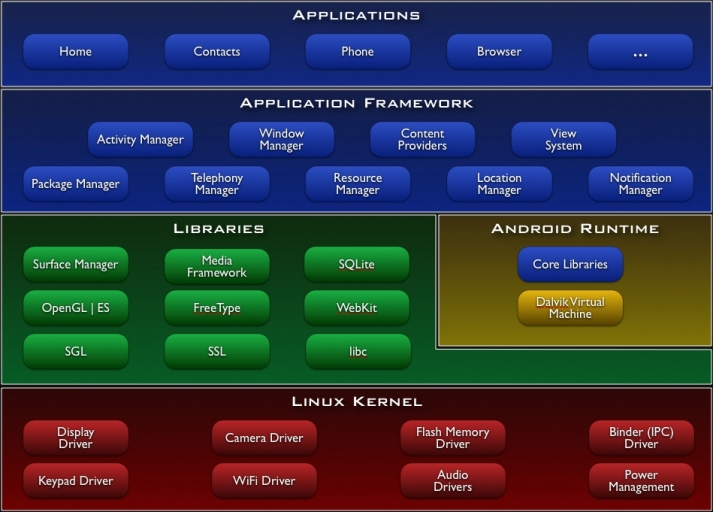
\includegraphics[scale=0.38]{images/a1.jpg}
\caption{Android Anatomy}
\label{fig:Anatomy}
\end{figure}

Apps provide multiple entry points.Android apps are built as a combination of distinct components that can be invoked individually. For instance, an individual activity provides a single screen for a userinterface, and a service independently performs work in the background. From one component you can start another component using an intent. You can even start a component in a different app, such as an activity in a maps app to show an
address. This model provides multiple entry points for a single app and allows any
app to behave as a user's "default" for an action that other apps may invoke.

Apps adapt to different devices, Android provides an adaptive app framework that allows you to provide unique resources for different device configurations. For example, you can create different XML layout les for different screen sizes and the system determines which layout
to apply based on the current device's screen size. You can query the availability of device features at runtime if any app features require specific hardware such as
a camera. If necessary, you can also declare features your app requires so app markets such as Google Play Store do not allow installation on devices that do not
support that feature Android comes with an Android market which is an online
software store. It was developed by Google.

 It allows Android users to select, and
download applications developed by third party developers and use them. There
are around 2.0 lack+ games, application and widgets available on the market for
users. Android applications are written in java programming language. Android is
available as open source for developers to develop applications which can be
further used for selling in android market. There are around 200000 applications
developed for android with over 3 billion+ downloads. Android relies on Linux version 2.6 for core system services such as security, memory management, process management, network stack, and driver model. For software development, Android provides Android SDK (Software development kit).

\subsection{Activity Lifecycle}
Activities in the system are managed as an activity stack. When a new activity
is started, it is placed on the top of the stack and becomes the running activitythe previous activity always remains below it in the stack, and will not come to
the foreground again until the new activity exits. An activity has essentially four
states:
If an activity in the foreground of the screen (at the top of the stack), it is
active or running.

If an activity has lost focus but is still visible (that is, a new non-full-sized or
transparent activity has focus on top of your activity), it is paused. A paused
activity is completely alive (it maintains all state and member information and
remains attached to the window manager), but can be killed by the system in
extreme low memory situations.
\begin{figure}[ht]
\centering
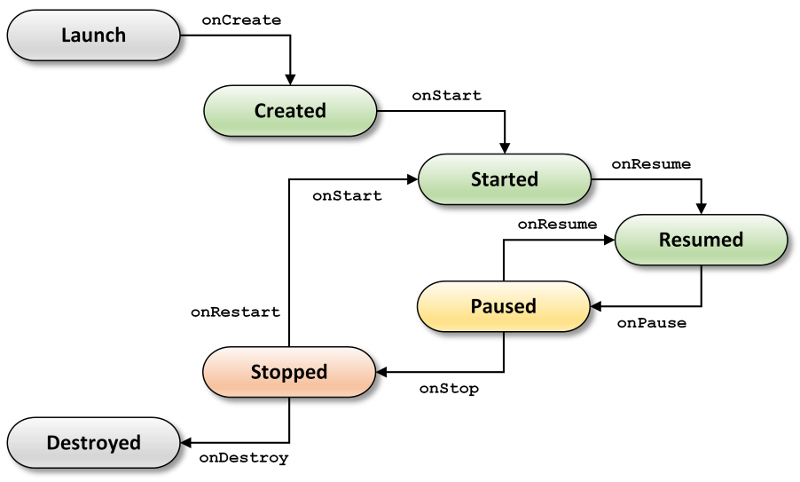
\includegraphics[scale=0.5]{images/a2.png}
\caption{Activity Life Cycle}
\label{fig: Activity }
\end{figure}

If an activity is completely obscured by another activity, it is stopped. It still
retains all state and member information, however, it is no longer visible to
the user so its window is hidden and it will often be killed by the system when
memory is needed elsewhere.

If an activity is paused or stopped, the system can drop the activity from memory by either asking it to finish, or simply killing its process. When it is displayed again to the user, it must be completely restarted and restored to its previous state.


\section{Libraries used in making this application}
\begin{itemize}
	\item \textbf{Android Support Library}
Android Support Library, Card View, Recycler View, Material : The application will
follow Material design guidelines.


\item \textbf{Realm}

Library to use Realm ORM in the application. This will allow to save data in
the database of the app and to retrieve, update and delete objects saved.\\

\item \textbf{Willian Charts}
Library to implement the graphics to show the statistics of the
app. Statistics include Expenses per month, per week and comparison of expenses according
to selected dates.



\end{itemize}


\subsection{Impliment UI for Each Activity and Fragment }
\begin{itemize}
	\item UI for MainActivity
\item UI for Expenses Activity
 \item UI for Expense Detail that will show last known expenses in the same category as a summary.
\item UI for Categories Fragment
\item UI for Statistics fragment
\end{itemize}

\begin{itemize}
	\item \textbf{Expenses Fragment}
Implement Business Logic for Adding and removing Expenses. Including removing from
recycler view:
\begin{itemize}
	\item Add expense or income
\item Remove expense or income from recycler view after enter to the detail page.
\end{itemize}

\item \textbf{Categories Fragment}
\begin{itemize}
	\item Categories add and remove from recycler view.
\item Detail of category with graph showing last used in the present week.
\end{itemize}



\item \textbf{Statistics Fragment}
Picker to select dates to make the query.
\begin{itemize}
	\item Show Graph for expenses made that month
\item Show graph for expenses made by category
\end{itemize}



\end{itemize}

\subsection{Any other supporting Language}
Java is a platform-independent programming language used to create secure
and robust application that may run on a single computer or may be distributed
among servers and clients over a network.

Java features such as platform-independency and portability ensure that while
de-veloping Java EE enterprise applications, you do not face the problems
related to hardware , network , and the operating system.

Java was started as a project called "Oak" by James Gosling in June 1991.
Gosling's goals were to implement a virtual machine and a language that had a
familiar C like notation but with greater uniformity and simplicity than C/C++.
The First publication of Java 1.0 was released by Sun Microsystems in 1995. It
made the promise of "Write Once, Run Anywhere", with free runtimes on
popular platforms. In 2006-2007 Sun released java as open source and
andplateform independent soft-ware. Over time new enhanced versions of Java
have been released. The current version of Java is Java 1.7 which is also
known as Java 7.he Java virtual machine (JVM) is a software implementation of
a computer that executes programs like a real machine. The Java virtual
machine is written specifically for a specific operating system, e.g. for Linux a
special implementation is required as well as for Windows.

Java programs are compiled by the Java compiler into bytecode. The Java
virtual machine interprets this bytecode and executes the Java program.
The Java runtime environment (JRE) consists of the JVM and the Java class li-
braries and contains the necessary functionality to start Java programs.
The JDK contains in addition the development tools necessary to create Java
pro-grams. The JDK consists therefore of a Java compiler, the Java virtual
machine, and the Java class libraries.

The characteristics and features of java are as follows :

\begin{itemize}
	\item \textbf{Simple}
Simple Java is a simple language because of its various features, Java
Doesn?t Support Pointers , Operator Overloading etc. It doesnt require
unreferenced object because java support automatic garbage collection.
Java provides bug free system due to the strong memory management.

\item \textbf{OOPS}
Object-Oriented Programming Language (OOPs) is the
methodology which provide software development and maintenance by
using
object
state,
behavior
Programming Lan-guage
must
,
and
have
properties.
the
Object Oriented following characteristics.
\begin{itemize}
	\item Encapsulation
\item Polymor-phism
 \item Inheritance
\item Abstraction

\end{itemize}
As the languages like Objective C, C++ fullls the above four characteristics yet
they are not fully object oriented lan-guages because they are structured
as well as object oriented languages.In java everything is an Object. Java
can be easily extended since it is based on the Object model.
\item \textbf{Secure}
Secure Java is Secure Language because of its many features it enables to
develop virus-free, tamper-free systems. Authentication techniques are
based on public-key encryption. Java does not support pointer explicitly for
the memory. All Program Run under the sandbox.

\item \textbf{Robust}
Robust Java was created as a strongly typed language. Data type issues
and problems are resolved at compile-time, and implicit casts of a variable
from one type to another are not allowed.
\item \textbf{Platform-independent}
Platform-independent Java Language is platform-independent due to its
hardware and software environment. Java code can be run on multiple
plat-forms e.g. windows, Linux, sun Solaris, Mac/Os etc. Java code is
compiled by the compiler and converted into byte code. This byte code is a
platform independent code because it can be run on multiple platforms i.e.
Write Once and Run Anywhere(WORA).
\item \textbf{Architectural Neural}
Architecture neutral It is not easy to write an application that can be used
on Windows , UNIX and a Macintosh. And its getting more complicated
with the move of windows to non Intel CPU architectures.
Java takes a diffierent approach. Because the Java compiler creates byte
code instructions that are subsequently interpreted by the java interpreter,
archi-tecture neutrality is achieved in the implementation of the java
interpreter for each new architecture.
\item \textbf{Portable}
Portable Java code is portable. It was an important design goal of Java that it
be portable so that as new architectures(due to hardware, operating system,
or both) are developed, the java environment could be ported to them.
In java, all primitive types(integers, longs, oats, doubles, and so on) are
20of de ned sizes, regardless of the machine or operating system on which
the program is run. This is in direct contrast to languages like C and C++
that leave the sized of primitive types up to the compiler and developer.
Additionally, Java is portable because the compiler itself is written in Java.
\item \textbf{Dynamic}
Dynamic Because it is interpreted , Java is an extremely dynamic language, At
runtime, the java environment can extends itself by linking in classes that may
be located on remote servers on a network(for example, the internet)
At runtime, the java interpreter performs name resolution while linking in the
necessary classes. The Java interpreter is also responsible for determining
the placement of object in memory. These two features of the Java interpreter
solve the problem of changing the de nition of a class used by other classes.
\item \textbf{Interpreted}
We all know that Java is an interpreted language as well. With
an interpreted language such as Java, programs run directly from the
source code.
The interpreter program reads the source code and translates it on the y
into computations. Thus, Java as an interpreted language depends on an
interpreter program.
The versatility of being platform independent makes Java to outshine from
other languages. The source code to be written and distributed is platform
independent.
Another advantage of Java as an interpreted language is its error
debugging quality. Due to this any error occurring in the program gets
traced. This is how it is di erent to work with Java.
\item \textbf{High performance}
High performance For all but the simplest or most infrequently used appli-cations,
performance is always a consideration for most applications, including
21graphics-intensive ones such as are commonly found on the world wide web,
the performance of java is more than adequate.
\item \textbf{Multithreading}
Writing a computer program that only does a single thing at a
time is an artificial constraint that lived with in most programming
languages. With java, we no longer have to live with this limitation. Support
for multiple, synchronized threads is built directly into the Java language
and runtime environment. Synchronized threads are extremely useful in
creating distributed, network-aware applications. Such as application may
be commu-nicating with a remote server in one thread while interacting
with a user in a different thread.
\item \textbf{Distributed}
Java facilitates the building of distributed application by a collection
of classes for use in networked applications. By using javas URL (Uniform
Resource Locator) class, an application can easily access a remote server.
Classes also are provided for establishing socket-level connections.


\end{itemize}



\subsection{Introduction to \LaTeX}
\begin{figure}[ht]
\centering

\includegraphics[scale=0.2]{images/latex.png}
\caption{\LaTeX{} Logo}
\end{figure}
\hspace{-1.8em} \LaTeX{}, I had never heard about this term before doing this project,
but when I came to know about it's features, it is just excellent. 
\LaTeX (pronounced /ˈleɪtɛk/, /ˈleɪtɛx/, /ˈlɑːtɛx/, or /ˈlɑːtɛk/) is a 
document markup language and document preparation system for the \TeX{} 
typesetting  program. Within the typesetting system, its name is styled 
as \LaTeX.
\begin{figure}[ht]
\centering
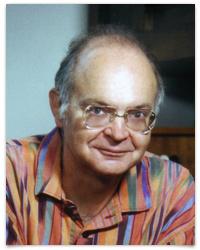
\includegraphics[scale=0.4]{images/donald.jpg}
\caption{Donald Knuth, Inventor Of \TeX{} typesetting system}
\end{figure}

\hspace{-1.8em} Within the typesetting system, its name is styled as \LaTeX. The term 
\LaTeX{} refers only to the language in which documents are written, 
not to the editor used to write those documents. In order to create a 
document in \LaTeX, a .tex file must be created using some form of text 
editor. While most text editors can be used to create a \LaTeX{} document, 
a number of editors have been created specifically for working with \LaTeX.\\

\noindent\LaTeX{} is most widely used by mathematicians, scientists, 
engineers, philosophers, linguists, economists and other scholars in 
academia. As a primary or intermediate format, e.g., translating DocBook 
and other XML-based formats to PDF, \LaTeX{} is used because of the 
high quality of typesetting achievable by \TeX. The typesetting system 
offers programmable desktop publishing features and extensive facilities 
for automating most aspects of typesetting and desktop publishing, 
including numbering and cross-referencing, tables and figures, 
page layout and bibliographies.\\

\noindent\LaTeX{} is intended to provide a high-level language that
accesses the power of \TeX. \LaTeX{} essentially comprises a
collection of \TeX{} macros and a program to process \LaTeX documents. 
Because the \TeX{} formatting commands are very low-level, it is usually 
much simpler for end-users to use \LaTeX{}.


\subsubsection{Typesetting}
\LaTeX{} is based on the idea that authors should be able to focus on 
the content of what they are writing without being distracted by its 
visual presentation. in preparing a \LaTeX{} document, the author 
specifies the logical structure using familiar concepts such as 
chapter, section, table, figure, etc., and lets the \LaTeX{} system 
worry about the presentation of these structures. it therefore 
encourages the separation of layout from content while still allowing 
manual typesetting adjustments where needed. 

\begin{verbatim}
\documentclass[12pt]{article}
\usepackage{amsmath}
\title{\LaTeX}
\begin{document}
  \maketitle 
  \LaTeX{} is a document preparation system 
  for the \TeX{} typesetting program.
   \par 
   $E=mc^2$
\end{document}
\end{verbatim}

\subsubsection{Installing \LaTeX{} on System}
Installation of \LaTeX{} on personal system is quite easy. As i have used \LaTeX{} on Ubuntu 13.04 so i am discussing the installation steps for Ubuntu 13.04 here:
\begin{itemize}
\item Go to terminal and type\\\\
\textit{sudo apt-get install texlive-full}
\item Your Latex will be installed on your system and you can check for manual page by typing.\\\\
\textit{man latex}\\

in terminal which gives manual for latex command.
\item To do very next step now one should stick this to mind that the document which one is going to produce is written in any type of editor whether it may be your most common usable editor Gedit or you can use vim by installing first vim into your system using command.\\\\
\textit{sudo apt-get install vim}
\item After you have written your document it is to be embedded with some set of commands that Latex uses so as to give a structure to your document. Note that whenever you wish your document to be looked into some other style just change these set of commands.
\item When you have done all these things save your piece of code with .tex format say test.tex. Go to terminal and type\\\\
\textit{latex path of the file test.tex Or pdflatex path of the file test.tex\\ eg: pdflatex test.tex}\\
for producing pdf file simultaneously.\\
After compiling it type command\\\\
\textit{evince filename.pdf\\ eg: evince test.pdf}\\
To see output pdf file. 
\end{itemize}

\subsubsection{Making Graphics in \LaTeX{}}
\LaTeX{} s also know popularly for making complex graphics. One such example is shown below here:\\
\begin{verbatim}
\documentclass{article}
\usepackage{tikz}
\usetikzlibrary{calendar,shadings}
\renewcommand*{\familydefault}{\sfdefault}
\colorlet{winter}{blue}
\colorlet{spring}{green!60!black}
\colorlet{summer}{orange}
\colorlet{fall}{red}
\newcount\mycount
\begin{document}
\begin{tikzpicture}[transform shape,
every day/.style={anchor=mid,font=\tiny}]
\node[circle,shading=radial,outer color=blue!30,inner color=white,
minimum width=15cm] {\textcolor{blue!80!black}{\Huge\the\year}};
\foreach \month/\monthcolor in
{1/winter,2/winter,3/spring,4/spring,5/spring,6/summer,
7/summer,8/summer,9/fall,10/fall,11/fall,12/winter} {
\mycount=\month
\advance\mycount by -1
\multiply\mycount by 30
\advance\mycount by -90
\shadedraw[shading=radial,outer color=\monthcolor!30,middle color=white,
inner color=white,draw=none] (\the\mycount:5.4cm) circle(1.4cm);
\calendar at (\the\mycount:5.4cm) [
dates=\the\year-\month-01 to \the\year-\month-last]
if (day of month=1) {\large\color{\monthcolor!50!black}\tikzmonthcode}
if (Sunday) [red]
if (all) {
\mycount=1
\advance\mycount by -\pgfcalendarcurrentday
\multiply\mycount by 11
\advance\mycount by 90
\pgftransformshift{\pgfpointpolar{\mycount}{1.2cm}}};}
\end{tikzpicture}
\end{document}
\end{verbatim}\\
%\begin{figure}[ht]
%\centering
%\includegraphics[scale=0.4]{images/3d.png}
%\caption{Graphics in \LaTeX{}}
%\end{figure}
\LaTeX{} with just invoking few additional packages.

\subsubsection{Pdfscreen \LaTeX{}}
There are some packages that can help to have unified document using \LaTeX{}. Example of such a package is pdfscreen that let the user view it’s document in two forms-print and screen. Print for hard copy and screen for viewing your document on screen. Download this package from www.ctan.org/tex-archive/macros/latex/contrib/pdfscreen/.\\
Then install it using above mention method.\\

\noindent To test it the test code is given below:-\\
Just changing print to screen gives an entirely different view. But for working of pdfscreen another package required are comment and fancybox.\\

\noindent The fancybox package provides several different styles of boxes for framing and rotating content in your document. Fancybox provides commands that produce square-cornered boxes with single or double lines, boxes with shadows, and round-cornered boxes with normal or bold lines. You can box mathematics, floats, center, flushleft, and flushright, lists, and pages.\\
 	
\noindent Whereas comments package selectively include/excludes portions of text. The comment package allows you to declare areas of a document to be included or excluded. One need to make these declarations in the preamble of your file. The package uses a method for exclusion that is pretty robust, and can cope with ill-formed bunches of text.\\

\noindent So these extra packages needed to be installed on system for the proper working of pdfscreen package.
\subsubsection{Web based graphic generation using \LaTeX{}}
\LaTeX{} is also useful when there is need of generating the graphics from browser. For
example to draw a circle by just entering its radius in html input box. So this kind
A
of project can be conveniently handled using \LaTeX{}. Basic idea behind this generation
process is that when user clicks on submit button after entering radius a script will run
that enter the radius in already made .tex file and recompiles it on server and makes its
pdf and postscript file. After that user can view those files by clicking on link provided
to view the files. See some screen shots of such a graphic generation project made by
Dr. H.S. Rai:\\
So here in the above input page which is also the index page user can enter input
for length of rectangle, breadth of rectangle and for radius of circle after that user can submit the values. After the values get submitted a script get runs by php code at server
side. This script first enters the dimensions of rectangle and circle that were selected by
user in to an already existing .tex file and replace with the older dimensions there. After
that script recompiles the the tex file and make it available for user.\\
	
\noindent In above figure it gets clear that .tex file has been compiled and pdf and postscript files
are available to user and user can download the graphics so produced. Hence graphics
can be generated in \LaTeX{} through web interface.

\subsection{Doxygen}
\begin{figure}[h]
	\centering 
\includegraphics[scale=1]{images/doxygen.jpg}
\end{figure}
Doxygen is a documentation generator, a tool for writing software reference documentation. The documentation is written within code, and is thus relatively easy to keep up to date. Doxygen can cross reference documentation and code, so that the reader of a document can easily refer to the actual code.
Doxygen supports multiple programming languages, especially C++, C, C\#, Objective-C, Java, Python, IDL, VHDL, Fortran and PHP.[2] Doxygen is free software, released under the terms of the GNU General Public License.

Doxygen is the de facto standard tool for generating documentation from annotated C++ sources, but it also supports other popular programming languages such as C, Objective-C, C\#, PHP, Java, Python, IDL (Corba, Microsoft, and UNO/OpenOffice flavors), Fortran, VHDL, Tcl, and to some extent.
Doxygen can help you in three ways:

\begin{itemize}
	\item It can generate an on-line documentation browser (in HTML) and/or an off-line reference manual (in ) from a set of documented source files. There is also support for generating output in RTF (MS-Word), PostScript, hyperlinked PDF, compressed HTML, and Unix man pages. The documentation is extracted directly from the sources, which makes it much easier to keep the documentation consistent with the source code.
	\item You can configure doxygen to extract the code structure from undocumented source files. This is very useful to quickly find your way in large source distributions. Doxygen can also visualize the relations between the various elements by means of include dependency graphs, inheritance diagrams, and collaboration diagrams, which are all generated automatically.
	\item You can also use doxygen for creating normal documentation (as I did for the doxygen user manual and web-site).
\end{itemize}

Doxygen looks at the file’s extension to determine how to parse a file. If a file has an .idl or .odl extension it is treated as an IDL file. If it has a .java extension it is treated as a file written in Java. Files ending with .cs are treated as C\# files and the .py extension selects the Python parser. Finally, files with the extensions .php, .php4, .inc or .phtml are treated as PHP sources. Any other extension is parsed as if it is a C/C++ file, where files that end with .m are treated as Objective-C source files.

If you start using doxygen for an existing project (thus without any documentation that doxygen is aware of), you can still get an idea of what the structure is and how the documented result would look like. To do so, you must set the EXTRACT ALL tag in the configuration file to YES. Then, doxygen will pretend everything in your sources is documented. Please note that as a consequence warnings about undocumented members will not be generated as long as EXTRACT ALL is set to YES.

To analyse an existing piece of software it is useful to cross-reference a (documented) entity with its definition in the source files. Doxygen will generate such cross-references if you set the SOURCE BROWSER tag to YES. It can also include the sources directly into the documentation by setting INLINE SOURCES to YES (this can be handy for code reviews for instance).

Doxygen is developed under Mac OS X and Linux, but is set-up to be highly portable. As a result, it runs on most other Unix flavors as well. Furthermore, executables for Windows are available.

\subsubsection{Features of Doxygen}
\begin{itemize}
	\item Requires very little overhead from the writer of the documentation. 
	Plain text will do, Markdown is support, and for more fancy or structured 
	output HTML tags and/or some of doxygen's special commands can be used.
	\item Cross platform: Works on Windows and many Unix flavors (including 
	Linux and Mac OS X).
	\item Comes with a GUI frontend (Doxywizard) to ease editing the options 
	and run doxygen. The GUI is available on Windows, Linux, and Mac OS X.
	\item Automatically generates class and collaboration diagrams in HTML 
	(as clickable image maps) and $\mbox{\LaTeX}$ (as Encapsulated PostScript 
	images).
	\item Allows grouping of entities in modules and creating a hierarchy 
	of modules.
	\item Doxygen can generate a layout which you can use and edit to change 
	the layout of each page.
	\item Can cope with large projects easily.
\end{itemize}
\subsubsection{Installation of Doxygen}
Doxygen can be installed using following commands:\\

\hspace{4pt} \$ git clone https://github.com/doxygen/doxygen.git\\ 

\hspace{4pt} \$ cd doxygen\\

\hspace{4pt} \$ ./configure\\

\hspace{4pt} \$ make \\


	\section{Validation}
	 	
\section{Expected hurdles}

\section{SDLC model to be used}


%\newpage

%\chapter{Technologies Used}
%
\section{Introduction to PHP}
\begin{figure}[h]
\centering \includegraphics[scale=0.4]{images/php.png}
\caption{Php logo}
\end{figure}
\noindent PHP is an open source server-side scripting language designed for Web development to produce dynamic Web pages. It is one of the first developed server-side scripting languages to be embedded into an HTML source document rather than calling an external file to process data. The code is interpreted by a Web server with a PHP processor module which generates the resulting Web page. It also has evolved to include a command-line interface capability and can be used in standalone graphical applications.\\

\noindent PHP can be deployed on most Web servers and also as a standalone shell on almost every operating system and platform, free of charge. A competitor to Microsoft’s Active Server Pages (ASP) server-side script engine and similar languages, PHP is installed on more than 20 million Web sites and 1 million Web servers. Notable software that uses PHP includes Drupal, Joomla, MediaWiki, and WordPress. PHP is a general-purpose scripting language.\\

\noindent It is especially suited to server-side web development where PHP generally runs on a web server. Any PHP code in a requested file is executed by the PHP runtime, usually to create dynamic web page content or dynamic images used on Web sites or elsewhere. It can also be used for command-line scripting and client-side graphical user interface (GUI) applications. PHP can be deployed on most Web servers, many operating systems.
\subsection{Features of PHP}
\begin{itemize}
\item Http Authentication
\item Cookies and Sessions
\item Connection Handling
\item Designer-friendly 
\item Cross platform Compatibility 
\item Loosely typed Language
\item Open Source
\item Easy code
\end{itemize}



\section{MySQL Database Server}
\begin{figure}[h]
\centering \includegraphics[scale=0.2]{images/mysql.jpg}
\caption{Mysql logo}
\end{figure}
\noindent I used the Mysql database for my project. It is world''s most popular open source database It 
is a relational database management system (RDBMS) that runs as a server 
providing multi-user access to a number of databases. It is named after 
developer Michael Widenius's daughter, My. The SQL phrase stands for
Structured Query Language. MySQL is written in C and C++.\\

\noindent Free-software-open source projects that require a 
full-featured database management system
often use MySQL. MySQL is also used in many high-profile, large-scale World 
Wide Web products, including
Wikipedia, Google (though not for searches) and Facebook.\\

\noindent MySQL is a popular choice of database for use in web 
applications, and is a central component of the widely used LAMP web 
application software LAMP is an acronym for “Linux, Apache, MySQL, 
Perl/PHP/Python”. MySQL is used in some of the most frequently visited web sites 
on the Internet, including Flickr, Nokia.com, YouTube, Wikipedia, Google 
and Facebook.\\

\noindent One of the greatest advantage of Django is that it synchronises the 
database only with one command withouut having any need to send 
different queries for insertion, deletion, updation etc. There is a 
file named models.py which is used for purpose of creating database.
\subsection{Features of MySQL}
\begin{itemize}
\item MySQL is a database management system.
\item MySQL is a relational database management system.
\item MySQL software is Open Source.
\item The MySQL Database Server is very fast, reliable, and easy to 
use.
\item MySQL Server works in client/server or embedded systems.
\item A large amount of contributed MySQL software is available.
\end{itemize}
\subsection{Installation of MySQL}
MySql can be installed using following commands:\\

\hspace{4pt} \$ sudo apt-get install mysql-server\\

\hspace{4pt} \$ sudo apt-get install mysql-client


\section{Introduction to Bootstrap} 

\begin{figure}[h]
\centering \includegraphics[scale=0.3]{images/bootstrap.png}
\caption{Bootstrap logo}
\end{figure}
\subsection{What is Bootstrap}
\noindent Bootstrap is a powerful front-end framework for faster and easier web development. It includes HTML and CSS based design templates for common user interface components like Typography, Forms, Buttons, Tables, Navigations, Dropdowns, Alerts, Modals, Tabs, Accordion, Carousel and many other as well as optional JavaScript extensions.
Bootstrap also gives you ability to create responsive layout with much less efforts.
\subsection{Advantages of Bootstrap}
The biggest advantage of using Bootstrap is that it comes with free set of tools for creating flexible and responsive web layouts as well as common interface components.
Additionally, using the Bootstrap data APIs you can create advanced interface components like Scrollspy and Typeaheads without writing a single line of JavaScript.
Here are some more advantages, why one should opt for Bootstrap:
\begin{itemize}
\item Save lots of time.
\item Responsive features.
\item Consistent design .
\item Easy to use.
\item Compatible with browsers.
\item Open Source.
\item Consistency.
\item Comprehensive List Of Components
\item Leveraging Javascript Libraries.
\item Frequent Updates.
\end{itemize}
\subsection{Installation of Bootstrap}
Downloading of Bootstrap is a very easy proccess.
Type the commands in the terminal:\\

 \$ git clone https://github.com/twbs/bootstrap.git\\


\noindent This will clone the bootstrap files on your pc/laptop and later u can use these files in your project.


\section{Introduction to Apache Web Server}

\begin{figure}[h]
\centering\includegraphics[scale=0.5]{images/apache.jpg}
\caption{Apache logo}
\end{figure}
\noindent Apache is a web server software notable for playing a key role in the initial 
growth of the World Wide Web. Apache is developed and maintained by an 
open community of developers under the auspices of the Apache Software 
Foundation. The application is available for a wide variety of operating 
systems, including Unix, FreeBSD, Linux, Solaris, Novell NetWare, Mac OS X, 
Microsoft Windows, OS/2, TPF, and eComStation. Released under the Apache 
License, Apache is open-source software.

\noindent The goal of this project is to provide a secure, efficient and extensible 
server that provides HTTP services in sync with the current HTTP standards.
\subsection{Features of Apache Server}
\begin{itemize}
\item Apache supports a variety of features, many implemented as compiled 
modules which extend the core functionality. These can range from 
server-side programming language support to authentication schemes. 
\item Apache features configurable error messages, DBMS-based 
authentication databases, and content negotiation. It is also supported 
by several graphical user interfaces (GUIs).
\item It supports password authentication and digital certificate 
authentication. Apache has a built in search engine and an HTML authorizing 
tool and supports FTP.
\end{itemize}

\subsection{Installation of Apache Server}
Apache web server can be installed using following commands:\\

\hspace{4pt} \$ sudo apt-get install apache2




%\section{Debconf}
%\input {input/debconf.tex}


\section{Introduction to Doxygen}
\input {input/doxygen.tex}


%\chapter{Experimental Results}
%\noindent Automated Building Drawings System is used to eliminate the previous manual process of creation of drawings using the traditional techniques by replacing it with the automated system, such that the end user can now easily make the required drawing design 
and the whole process can be made more easy and reliable for the users thus saving time. All the drawings can also be exported in some supported file format using this software thus making the system more useful and reliable.\\

\noindent User can easily maintain all the record of the previously created drawing designs by saving them into the computer memory. It eliminates the manual operations and thus
increases productivity in the system by automating it. Entities can be crated just by giving their names and parameters thus the whole process becomes a very fast. The Drawing can be easily generated for a particular building by giving all the specifications such as length of the walls, height, width etc thus managing the system overall. \\

\noindent Firstly the user input the required specifications of the desired design such as length, height, the type of entity etc. Then these parameters and all other details are saved in a input file which is a txt file. Then this file is parsed into the system where the processing is done and the input file is splitted into the output file where its parameters are separated into the lines. \\

\noindent This file then parsed into the system from which the system reads the content that is specified by the user and then according to that information the Automated Building Drawings system produces a drawing which can be opened using the cad software LibreCad.\\

\noindent The traditional pencil and paper work can be reduced to a great extent by doing work using this software and saving paper thus
making it environment friendly. Thus, making it automated process. Lot of time was wasted during the drawing of buildings using the pencil and paper. So with this software even the  people who is not proficient in computer can easily take the benefit of cration of drawings using this software.


\section{Testing}
The most important activity at the implementation stage is the system testing with the objective of validating the system against the designed criteria. During the development cycle, user was involved in all the phases that are analysis, design and coding. After each phase the user was asked whether he was satisfied with the output and the desired rectification was done at the moment. During coding, generally bottom up technique is used. Firstly the lower level modules are coded and then they are integrated together.

Software testing is an investigation conducted to provide stakeholders with information about the quality of the product or service under test.Software testing can also provide an objective, independent view of the software to allow the business to appreciate and understand the risks of software implementation. Test techniques include the process of executing a program or application with the intent of finding software bugs (errors or other defects). Software testing involves the execution of a software component or system component to evaluate one or more properties of interest. In general, these properties indicate the extent to which the component or system under test:
\begin{itemize}
	\item meets the requirements that guided its design and development,
	\item responds correctly to all kinds of inputs,
	\item performs its functions within an acceptable time,
	is sufficiently usable,
	\item can be installed and run in its intended environments, and achieves the general result its stakeholders desire.
\end{itemize}

As the number of possible tests for even simple software components is practically infinite, all software testing uses some strategy to select tests that are feasible for the available time and resources. As a result, software testing typically (but not exclusively) attempts to execute a program or application with the intent of finding software bugs (errors or other defects). The job of testing is an iterative process as when one bug is fixed, it can illuminate other, deeper bugs, or can even create new ones.

Software testing can provide objective, independent information about the quality of software and risk of its failure to users and/or sponsors.
Software testing can be conducted as soon as executable software (even if partially complete) exists. The overall approach to software development often determines when and how testing is conducted. For example, in a phased process, most testing occurs after system requirements have been defined and then implemented in testable programs. In contrast, under an Agile approach, requirements, programming, and testing are often done concurrently.

Thus before implementation, it involves the testing of the system. The testing phase involves testing first of separate parts of the system and then finally of the system as a whole. Each independent module is tested first and then the complete system is tested. This is the most important phase of the system development. The user carries out this testing and test data is also prepared by the user to check for all possible combinations of correct data as well as the wrong data that is trapped by the system. So the testing phase consists of the following steps:

\subsection{Unit Testing}
In the bottom of coding technique, each module is tested individually. Firstly the module is tested with some test data that covers all the possible paths and then the actual data was fed to check for results.Unit testing, also known as component testing, refers to tests that verify the functionality of a specific section of code, usually at the function level. In an object-oriented environment, this is usually at the class level, and the minimal unit tests include the constructors and destructors.

These types of tests are usually written by developers as they work on code (white-box style), to ensure that the specific function is working as expected. One function might have multiple tests, to catchcorner cases or other branches in the code. Unit testing alone cannot verify the functionality of a piece of software, but rather is used to ensure that the building blocks of the software work independently from each other.

Unit testing is a software development process that involves synchronized application of a broad spectrum of defect prevention and detection strategies in order to reduce software development risks, time, and costs. It is performed by the software developer or engineer during the construction phase of the software development lifecycle. Rather than replace traditional QA focuses, it augments it. Unit testing aims to eliminateconstruction errors before code is promoted to QA; this strategy is intended to increase the quality of the resulting software as well as the efficiency of the overall development and QA process.

Depending on the organization's expectations for software development, unit testing might include static code analysis, data-flow analysis, metrics analysis, peer code reviews, code coverage analysis and other software verification practices.

\subsection{Integration Testing}
After all the modules are ready and duly tested, these have to be integrated into the application. This integrated application was again tested first with the test data and then with the actual data.

Integration testing is any type of software testing that seeks to verify the interfaces between components against a software design. Software components may be integrated in an iterative way or all together ("big bang"). Normally the former is considered a better practice since it allows interface issues to be located more quickly and fixed.

Integration testing, also known as integration and testing (I\&T), is a softwaredevelopment process which program units are combined and tested as groups in multiple ways. In this context, a unit is defined as the smallest testable part of anapplication. Integration testing can expose problems with the interfaces among program components before trouble occurs in real-world program execution. Integration testing is a component of Extreme Programming (XP), a pragmatic method of software development that takes a meticulous approach to building a product by means of continual testing and revision.
Once all the individual units are created and tested, we start combining those “Unit Tested” modules and start doing the integrated testing. So the meaning of Integration testing is quite straight forward- Integrate/combine the unit tested module one by one and test the behaviour as a combined unit.

The main function or goal of Integration testing is to test the interfaces between the units/modules.
The individual modules are first tested in isolation. Once the modules are unit tested, they are integrated one by one, till all the modules are integrated, to check the combinational behavior, and validate whether the requirements are implemented correctly or not.
Here we should understand that, Integration testing does not happens at the end of the cycle, rather it is conducted simultaneously with the development. So in most of the times all the modules are not actually available to test and here is what the challenge comes to test something which does not exists!

Integration testing works to expose defects in the interfaces and interaction between integrated components (modules). Progressively larger groups of tested software components corresponding to elements of the architectural design are integrated and tested until the software works as a system.

\subsection{Parallel Testing}
The third in the series of tests before handling over the system to the user is the parallel processing of the old and the new system. At this stage, complete and thorough testing is done and supports out the event that goes wrong. This provides the better practical support to the persons using the system for the first time who may be uncertain or even nervous using it.

Parallel testing is a testing technique in which the same inputs are entered in two different versions of the application and reporting the anomalies. Since the system that is being tested will be the new means by which payroll is calculated, parallel testing should be managed by those who will be regularly taking care of payroll responsibilities. This allows hands-on training and generates invaluable troubleshooting experience before the system even goes live. Unfortunately, this usually doubles the workload for these employees that have to enter payroll information into both the new and old system, so additional help may be needed during this transition phase. When needed, managers within the organization that have more experience with the new system or vendor representatives may help to answer questions and provide information.

Executing test runs in parallel is obviously very important if many test runs need to be executed. The goal is to exploit the available resources as well as possible. If several machines are available, the goal is to achieve linear speedup; that is, the running time of executing all tests decreases linearly with the number of machines. In order to achieve this speed-up, it is important to balance the load on all machines – just as in all parallel applications .At the same time, however, it is also important to control the state of the test database(s) and to execute the test runs in such a way that the number of database reset operations is minimized – just as for non-parallel testing in .As a result, parallel testing involves solving a two-dimensional optimization problem: (a) partitioning: deciding which test runs to execute on which machine; and (b) ordering: deciding in which order to execute the test runs on each machine.

Parallel testing is a two dimensional scheduling problem. In addition to deciding in which order to execute the test runs, a scheduling strategy must partition the test runs. Depending on the architecture, Shared-Database or Shared-Nothing (see below), a parallel execution can increase the number of resets due to interference (Shared-Database) or decrease the number of resets (Shared-Nothing) by executing test runs that are in conflict concurrently. As a result, conflict information ought to be taken into account in order to decide on which machine to execute which test run. 

Furthermore, it is important to balance the load on all machines so that the resources are used as well as possible. Load balancing can be carried out without conflict information; load balancing should be carried out taking the current load of machines and the estimated length of test runs into account.

\chapter{System Design}

\section{Screenshots}

The basic requirement of this app is that the user must be having ANDROID
Operating System in his phone or tablet. The minimum version of Androids Operating
System must be ICECREAM SANDWICH. All the versions of Android OS above
IcecreamSandwich( i.e. Jellybean, Kitkat, Lollipop,Marshmallows) will support this
app. A user needs Monitary app installed in device .


\noindent As shown in the Figure \ref{fig:1}, .\\Brief introduction showing the features available in the application.

\begin{figure}[ht]
\centering
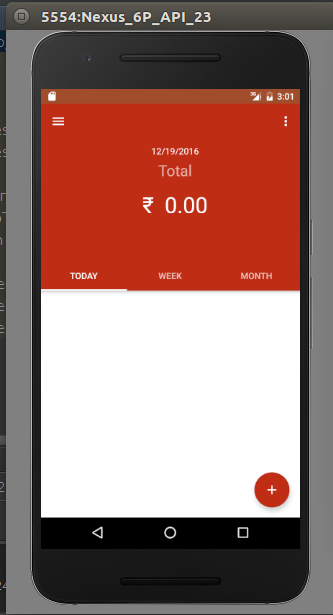
\includegraphics[scale=0.5]{images/s1.png}
\caption{Screen 1}
\label{fig:1}
\end{figure}

\noindent This are the options the navigation drawer the app will contain. These will contain the screens the user can navigate too that can be seen in Figure \ref{fig:2}. \\

\begin{figure}[ht]
	\centering
	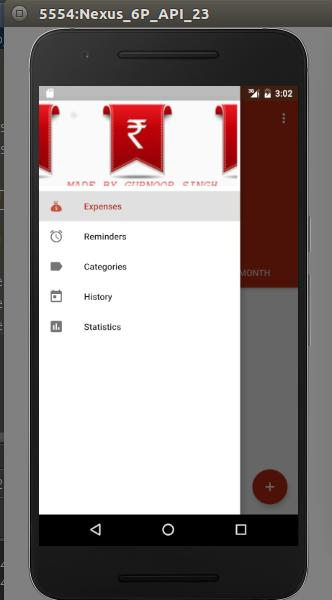
\includegraphics[scale=0.49]{images/s2.png}
	\caption{Screen 2}
	\label{fig:2}
\end{figure}

\noindent  Statistics will be able to change according to the dates selected. Default values will be the current week. User Will be able to see diagrams according to Quantity and
days, Quantity and categories and others.as seen in the Figure \ref{fig:3}.\\

\begin{figure}[ht]
\centering
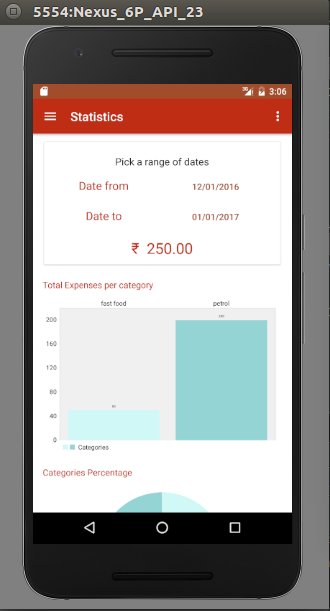
\includegraphics[scale=0.5]{images/s3.png}
\caption{Screen 3}
\label{fig:3}
\end{figure}

\noindent Reminder view will contain details from the reminder created and the user can edit
the reminder values. in Figure \ref{fig:4}. \\

\begin{figure}[ht]
\centering
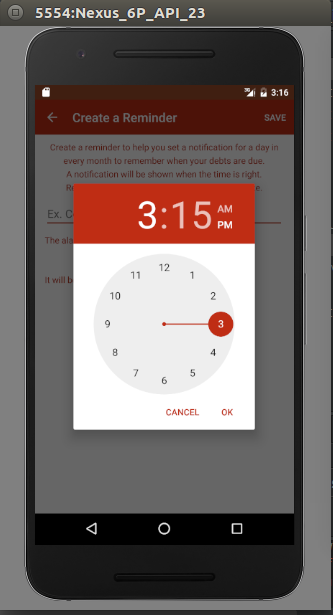
\includegraphics[scale=0.38]{images/s4.png}
\caption{Screen 4}
\label{fig:4}
\end{figure}

\noindent Reminder screen will show the current saved Reminder and if they are active or not.
To activate one it will have a switch next to the name so it can be activated in any
moment. The user will be able to erase and add from this view as seen in the Figure \ref{fig:5}. It's named as output.dxf. We can open that file in LibreCAD directly from the command-line.\\


\begin{figure}[ht]
\centering
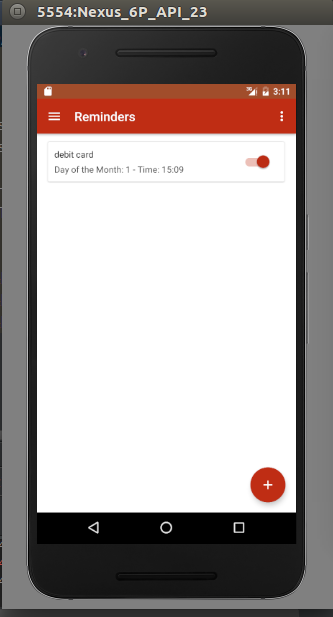
\includegraphics[scale=0.5]{images/s6.png}
\caption{Screen 5}
\label{fig:5}
\end{figure}

\noindent Expenses View is the main screen that will be showed. The user will be able to add expenses and see a total amount in Today, Week and Month. as shown in Figure \ref{fig:6}. 

\begin{figure}[ht]
\centering
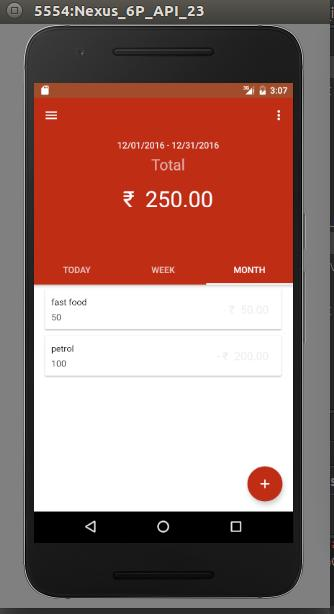
\includegraphics[scale=0.38]{images/s61.png}
\caption{Screen 6}
\label{fig:6}
\end{figure}

\noindent This activity will provide necessary help to the user. One can also mail the maker
(GURNOOR SINGH) for further queries as shown in Figure \ref{fig:7}. 

\begin{figure}[ht]
\centering
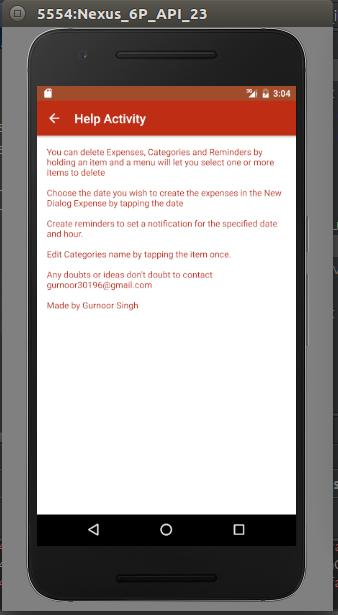
\includegraphics[scale=0.38]{images/s7.png}
\caption{Screen 7}
\label{fig:7}
\end{figure}
\noindent User will be able to add and delete categories from the Categories View \ref{fig:8}. 

\begin{figure}[ht]
\centering
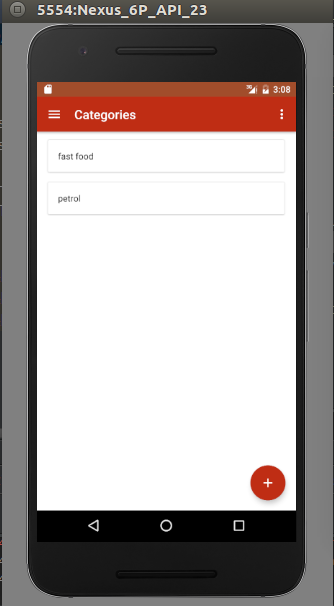
\includegraphics[scale=0.38]{images/s8.png}
\caption{Screen 8}
\label{fig:8}
\end{figure}


\chapter{Implementation ,Testing and Maintenance}
\section{Introduction to Languages,IDE’s,Tools and Technologies used for Implementation}
	
\subsection{Technologies used}

\subsubsection{Firebase}

Firebase helps you build better mobile apps and grow your business.

Firebase is a mobile platform from Google offering a number of different features that you can pick ‘n mix from. Specifically, these features revolve around cloud services, allowing users to save and retrieve data to be accessed from any device or browser. This can be useful for such things as cloud messaging, hosting, crash reporting, notifications, analytics and even earning money through AdMob.

It works with Android apps, iOS apps and web apps and best of all: it’s free!

\begin{itemize}

\item \textbf{Setting up a project}

Before you can do anything with Firebase, you first need to create an account. You can do this over at firebase.google.com.

\begin{figure}[ht]
\centering
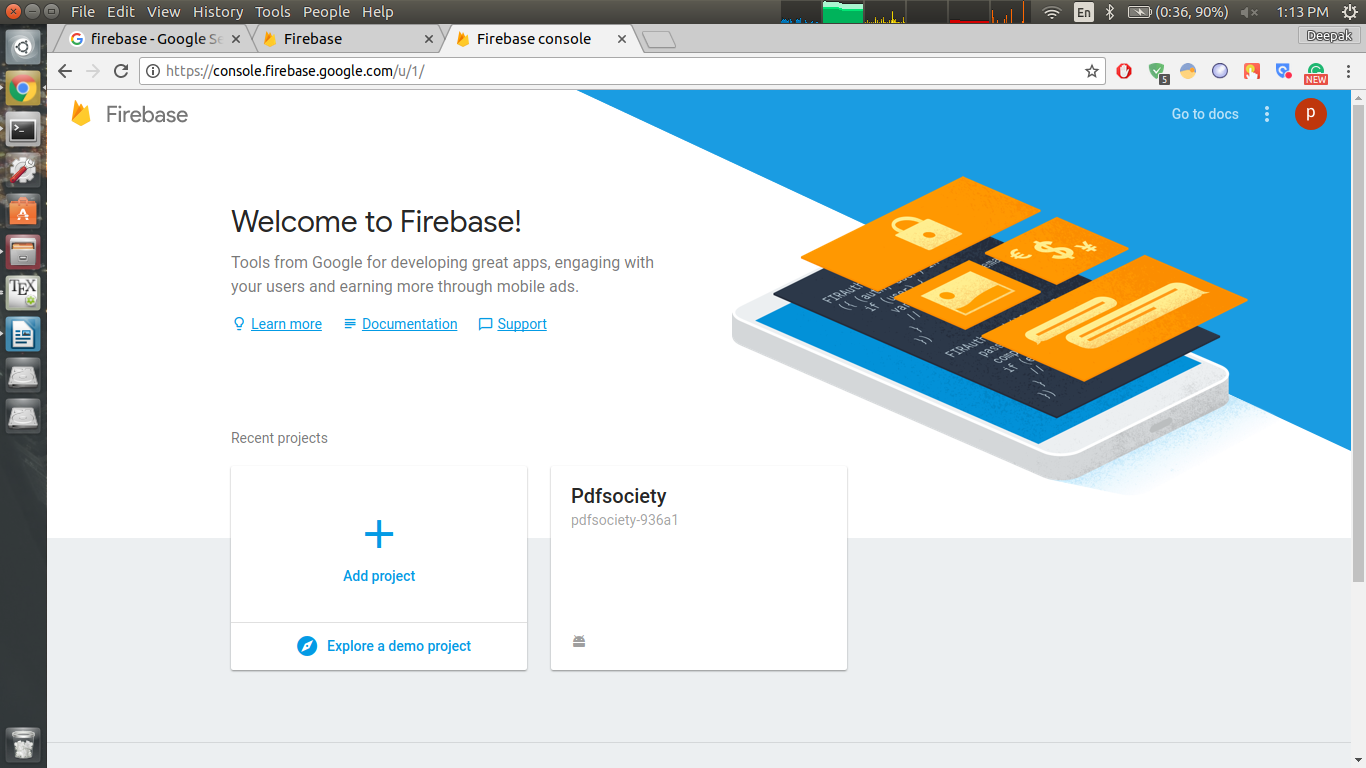
\includegraphics[scale=0.20]{images/Pdf2.png}
\caption{Firebase Console}
\end{figure}

 

\item \textbf{Firebase Products}

\begin{figure}[ht]
\centering
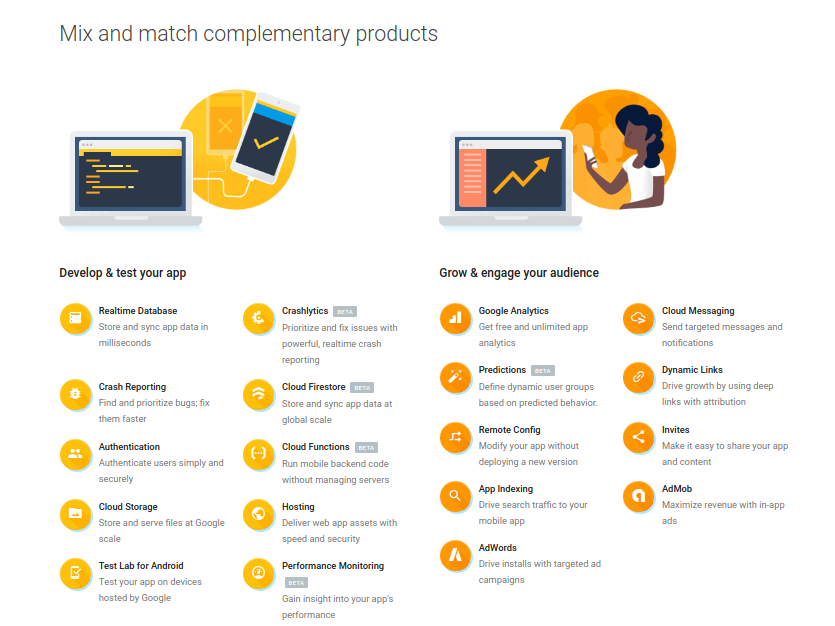
\includegraphics[scale=0.4]{images/Pdf1.png}
\caption{Firebase Products}
\end{figure}

\begin{itemize}

\item \textbf{Firebase Authentication}

Firebase Authentication aims to make building secure authentication systems easy, while improving the sign-in and onboarding experience for end users. It provides an end-to-end identity solution, supporting email and password accounts, phone auth, and Google, Twitter, Facebook, and GitHub login, and more.

Most apps need to know the identity of a user. Knowing a user's identity allows an app to securely save user data in the cloud and provide the same personalized experience across all of the user's devices.
Firebase Authentication provides backend services, easy-to-use SDKs, and ready-made UI libraries to authenticate users to your app. It supports authentication using passwords, phone numbers, popular federated identity providers like Google, Facebook and Twitter, and more.

Firebase Authentication integrates tightly with other Firebase services, and it leverages industry standards like OAuth 2.0 and OpenID Connect, so it can be easily integrated with your custom backend.

\item \textbf{Firebase Realtime Database}

Store and sync data with our NoSQL cloud database. Data is synced across all clients in realtime, and remains available when your app goes offline.

The Firebase Realtime Database is a cloud-hosted database. Data is stored as JSON and synchronized in realtime to every connected client. When you build cross-platform apps with our iOS, Android, and JavaScript SDKs, all of your clients share one Realtime Database instance and automatically receive updates with the newest data.


\item \textbf{Cloud Storage}

Cloud Storage is built for app developers who need to store and serve user-generated content, such as photos or videos.

Cloud Storage for Firebase is a powerful, simple, and cost-effective object storage service built for Google scale. The Firebase SDKs for Cloud Storage add Google security to file uploads and downloads for your Firebase apps, regardless of network quality. You can use our SDKs to store images, audio, video, or other user-generated content. On the server, you can use Google Cloud Storage, to access the same files.
	\end{itemize}
	\end{itemize}
	
\subsubsection{Android}


Android provides a rich application framework that allows you to build innovative
apps and games for mobile devices in a Java language environment. The documents
listed in the left navigation provide details about how to build apps using Android's
various APIs.The various fundamental concepts about the Android app framework:

\begin{figure}[ht]
\centering
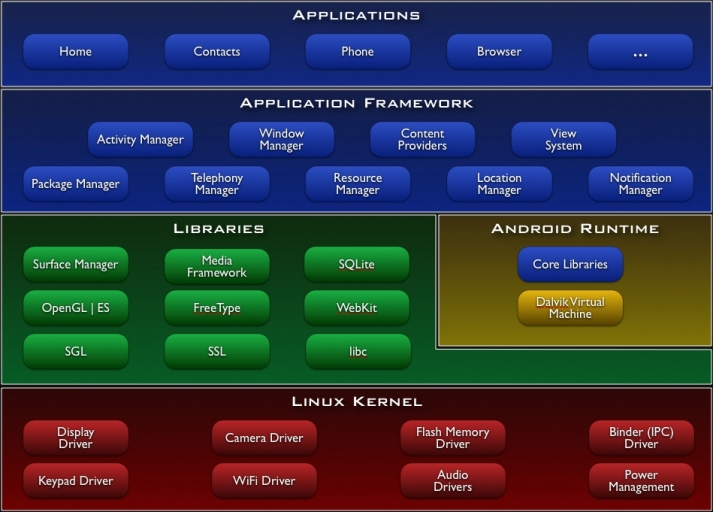
\includegraphics[scale=0.38]{images/a1.jpg}
\caption{Android Anatomy}
\label{fig:Anatomy}
\end{figure}

Apps provide multiple entry points.Android apps are built as a combination of distinct components that can be invoked individually. For instance, an individual activity provides a single screen for a userinterface, and a service independently performs work in the background. From one component you can start another component using an intent. You can even start a component in a different app, such as an activity in a maps app to show an
address. This model provides multiple entry points for a single app and allows any
app to behave as a user's "default" for an action that other apps may invoke.

Apps adapt to different devices, Android provides an adaptive app framework that allows you to provide unique resources for different device configurations. For example, you can create different XML layout les for different screen sizes and the system determines which layout
to apply based on the current device's screen size. You can query the availability of device features at runtime if any app features require specific hardware such as
a camera. If necessary, you can also declare features your app requires so app markets such as Google Play Store do not allow installation on devices that do not
support that feature Android comes with an Android market which is an online
software store. It was developed by Google.

 It allows Android users to select, and
download applications developed by third party developers and use them. There
are around 2.0 lack+ games, application and widgets available on the market for
users. Android applications are written in java programming language. Android is
available as open source for developers to develop applications which can be
further used for selling in android market. There are around 200000 applications
developed for android with over 3 billion+ downloads. Android relies on Linux version 2.6 for core system services such as security, memory management, process management, network stack, and driver model. For software development, Android provides Android SDK (Software development kit).

\begin{itemize}

\item \textbf{Activity Lifecycle}
Activities in the system are managed as an activity stack. When a new activity
is started, it is placed on the top of the stack and becomes the running activitythe previous activity always remains below it in the stack, and will not come to
the foreground again until the new activity exits. An activity has essentially four
states:
If an activity in the foreground of the screen (at the top of the stack), it is
active or running.

If an activity has lost focus but is still visible (that is, a new non-full-sized or
transparent activity has focus on top of your activity), it is paused. A paused
activity is completely alive (it maintains all state and member information and
remains attached to the window manager), but can be killed by the system in
extreme low memory situations.
\begin{figure}[ht]
\centering
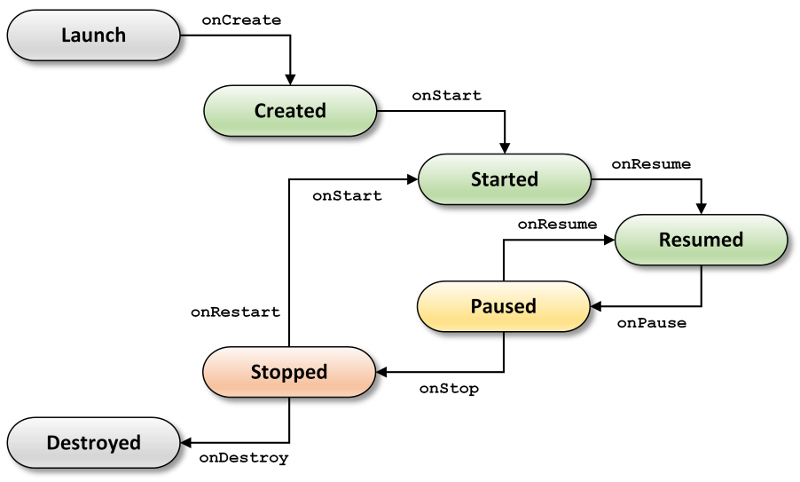
\includegraphics[scale=0.5]{images/a2.png}
\caption{Activity Life Cycle}
\label{fig: Activity }
\end{figure}

If an activity is completely obscured by another activity, it is stopped. It still
retains all state and member information, however, it is no longer visible to
the user so its window is hidden and it will often be killed by the system when
memory is needed elsewhere.

If an activity is paused or stopped, the system can drop the activity from memory by either asking it to finish, or simply killing its process. When it is displayed again to the user, it must be completely restarted and restored to its previous state.


\item \textbf{Libraries used in making this application}

\begin{itemize}
	\item \textbf{Android Support Library}
Android Support Library, Card View, Recycler View, Material : The application will
follow Material design guidelines.

\end{itemize}

\end{itemize}

\subsection{Language used}
\subsubsection{JAVA}

Java is a platform-independent programming language used to create secure
and robust application that may run on a single computer or may be distributed
among servers and clients over a network.

Java features such as platform-independency and portability ensure that while
de-veloping Java EE enterprise applications, you do not face the problems
related to hardware , network , and the operating system.

Java was started as a project called "Oak" by James Gosling in June 1991.
Gosling's goals were to implement a virtual machine and a language that had a
familiar C like notation but with greater uniformity and simplicity than C/C++.
The First publication of Java 1.0 was released by Sun Microsystems in 1995. It
made the promise of "Write Once, Run Anywhere", with free runtimes on
popular platforms. In 2006-2007 Sun released java as open source and
andplateform independent soft-ware. Over time new enhanced versions of Java
have been released. The current version of Java is Java 1.7 which is also
known as Java 7.he Java virtual machine (JVM) is a software implementation of
a computer that executes programs like a real machine. The Java virtual
machine is written specifically for a specific operating system, e.g. for Linux a
special implementation is required as well as for Windows.

Java programs are compiled by the Java compiler into bytecode. The Java
virtual machine interprets this bytecode and executes the Java program.
The Java runtime environment (JRE) consists of the JVM and the Java class li-
braries and contains the necessary functionality to start Java programs.
The JDK contains in addition the development tools necessary to create Java
pro-grams. The JDK consists therefore of a Java compiler, the Java virtual
machine, and the Java class libraries.

The characteristics and features of java are as follows :

\begin{itemize}
	\item \textbf{Simple}
Simple Java is a simple language because of its various features, Java
Doesn?t Support Pointers , Operator Overloading etc. It doesnt require
unreferenced object because java support automatic garbage collection.
Java provides bug free system due to the strong memory management.

\item \textbf{OOPS}
Object-Oriented Programming Language (OOPs) is the
methodology which provide software development and maintenance by
using
object
state,
behavior
Programming Lan-guage
must
,
and
have
properties.
the
Object Oriented following characteristics.
\begin{itemize}
	\item Encapsulation
\item Polymor-phism
 \item Inheritance
\item Abstraction

\end{itemize}
As the languages like Objective C, C++ fullls the above four characteristics yet
they are not fully object oriented lan-guages because they are structured
as well as object oriented languages.In java everything is an Object. Java
can be easily extended since it is based on the Object model.
\item \textbf{Secure}
Secure Java is Secure Language because of its many features it enables to
develop virus-free, tamper-free systems. Authentication techniques are
based on public-key encryption. Java does not support pointer explicitly for
the memory. All Program Run under the sandbox.

\item \textbf{Robust}
Robust Java was created as a strongly typed language. Data type issues
and problems are resolved at compile-time, and implicit casts of a variable
from one type to another are not allowed.
\item \textbf{Platform-independent}
Platform-independent Java Language is platform-independent due to its
hardware and software environment. Java code can be run on multiple
plat-forms e.g. windows, Linux, sun Solaris, Mac/Os etc. Java code is
compiled by the compiler and converted into byte code. This byte code is a
platform independent code because it can be run on multiple platforms i.e.
Write Once and Run Anywhere(WORA).
\item \textbf{Architectural Neural}
Architecture neutral It is not easy to write an application that can be used
on Windows , UNIX and a Macintosh. And its getting more complicated
with the move of windows to non Intel CPU architectures.
Java takes a diffierent approach. Because the Java compiler creates byte
code instructions that are subsequently interpreted by the java interpreter,
archi-tecture neutrality is achieved in the implementation of the java
interpreter for each new architecture.
\item \textbf{Portable}
Portable Java code is portable. It was an important design goal of Java that it
be portable so that as new architectures(due to hardware, operating system,
or both) are developed, the java environment could be ported to them.
In java, all primitive types(integers, longs, oats, doubles, and so on) are
20of de ned sizes, regardless of the machine or operating system on which
the program is run. This is in direct contrast to languages like C and C++
that leave the sized of primitive types up to the compiler and developer.
Additionally, Java is portable because the compiler itself is written in Java.
\item \textbf{Dynamic}
Dynamic Because it is interpreted , Java is an extremely dynamic language, At
runtime, the java environment can extends itself by linking in classes that may
be located on remote servers on a network(for example, the internet)
At runtime, the java interpreter performs name resolution while linking in the
necessary classes. The Java interpreter is also responsible for determining
the placement of object in memory. These two features of the Java interpreter
solve the problem of changing the de nition of a class used by other classes.
\item \textbf{Interpreted}
We all know that Java is an interpreted language as well. With
an interpreted language such as Java, programs run directly from the
source code.
The interpreter program reads the source code and translates it on the y
into computations. Thus, Java as an interpreted language depends on an
interpreter program.
The versatility of being platform independent makes Java to outshine from
other languages. The source code to be written and distributed is platform
independent.
Another advantage of Java as an interpreted language is its error
debugging quality. Due to this any error occurring in the program gets
traced. This is how it is di erent to work with Java.
\item \textbf{High performance}
High performance For all but the simplest or most infrequently used appli-cations,
performance is always a consideration for most applications, including
21graphics-intensive ones such as are commonly found on the world wide web,
the performance of java is more than adequate.
\item \textbf{Multithreading}
Writing a computer program that only does a single thing at a
time is an artificial constraint that lived with in most programming
languages. With java, we no longer have to live with this limitation. Support
for multiple, synchronized threads is built directly into the Java language
and runtime environment. Synchronized threads are extremely useful in
creating distributed, network-aware applications. Such as application may
be commu-nicating with a remote server in one thread while interacting
with a user in a different thread.
\item \textbf{Distributed}
Java facilitates the building of distributed application by a collection
of classes for use in networked applications. By using javas URL (Uniform
Resource Locator) class, an application can easily access a remote server.
Classes also are provided for establishing socket-level connections.


\end{itemize}

\subsubsection{XML}
Extensible Markup Language (XML) is a markup language that defines a set of rules for encoding documents in a format that is both human-readable and machine-readable through use of tags that can be created and defined by users. Much like natural language is extensible (that is, can grow) when speakers create new words and agree on what they mean, XML is a markup language that can grow when users create new elements and agree on what they mean. For example, XML can markup machine-readably that apples and bananas are types of fruit, which is semantically deeper than the purpose of HTML. However, HTML is useful for display of content; often HTML is used to display XML content after transformation with XSL.

\subsection{IDE used}
\subsubsection{Android Studio}

\begin{figure}[ht]
\centering

\includegraphics[scale=0.38]{images/android.png}
\caption{Android Studio}
\end{figure}

Android Studio is the official integrated development environment (IDE) for Google's Android operating system, built on JetBrains' IntelliJ IDEA software and designed specifically for Android development.
It is available for download on Windows, macOS and Linux based operating systems. It is a replacement for the Eclipse Android Development Tools (ADT) as primary IDE for native Android application development. 

Android Studio was announced on May 16, 2013 at the Google I/O conference. It was in early access preview stage starting from version 0.1 in May 2013, then entered beta stage starting from version 0.8 which was released in June 2014. The first stable build was released in December 2014, starting from version 1.0. The current stable version is 2.3.3, released in June 2017. Next major update, version 3.0, is in preview stage as of September 2017.

It offer tools custom-tailored for Android developers, including rich code editing, debugging, testing, and profiling tools.




\begin{itemize}
\item \textbf{System Requirements}
Android application development on either of the following operating systems −
\vskip 0.1in

Microsoft Windows 10/8/7/Vista/2003 (32 or 64-bit)
\\Mac OS X 10.8.5 or higher, up to 10.9 (Mavericks)
\\GNOME or KDE desktop
\vskip 0.1in

Second point is that all the required tools to develop Android applications are open source and can be downloaded from the Web. Following is the list of software's you will need before you start your Android application programming.\\

Java JDK5 or later version
\\Java Runtime Environment (JRE) 6
\\Android Studio
\end{itemize}

\subsection{Introduction to \LaTeX}
\begin{figure}[ht]
\centering

\includegraphics[scale=0.2]{images/latex.png}
\caption{\LaTeX{} Logo}
\end{figure}
\hspace{-1.8em} \LaTeX{}, I had never heard about this term before doing this project,
but when I came to know about it's features, it is just excellent. 
\LaTeX (pronounced /ˈleɪtɛk/, /ˈleɪtɛx/, /ˈlɑːtɛx/, or /ˈlɑːtɛk/) is a 
document markup language and document preparation system for the \TeX{} 
typesetting  program. Within the typesetting system, its name is styled 
as \LaTeX.

\hspace{-1.8em} Within the typesetting system, its name is styled as \LaTeX. The term 
\LaTeX{} refers only to the language in which documents are written, 
not to the editor used to write those documents. In order to create a 
document in \LaTeX, a .tex file must be created using some form of text 
editor. While most text editors can be used to create a \LaTeX{} document, 
a number of editors have been created specifically for working with \LaTeX.\\

\noindent\LaTeX{} is most widely used by mathematicians, scientists, 
engineers, philosophers, linguists, economists and other scholars in 
academia. As a primary or intermediate format, e.g., translating DocBook 
and other XML-based formats to PDF, \LaTeX{} is used because of the 
high quality of typesetting achievable by \TeX. The typesetting system 
offers programmable desktop publishing features and extensive facilities 
for automating most aspects of typesetting and desktop publishing, 
including numbering and cross-referencing, tables and figures, 
page layout and bibliographies.\\

\noindent\LaTeX{} is intended to provide a high-level language that
accesses the power of \TeX. \LaTeX{} essentially comprises a
collection of \TeX{} macros and a program to process \LaTeX documents. 
Because the \TeX{} formatting commands are very low-level, it is usually 
much simpler for end-users to use \LaTeX{}.


\subsubsection{Typesetting}
\LaTeX{} is based on the idea that authors should be able to focus on 
the content of what they are writing without being distracted by its 
visual presentation. in preparing a \LaTeX{} document, the author 
specifies the logical structure using familiar concepts such as 
chapter, section, table, figure, etc., and lets the \LaTeX{} system 
worry about the presentation of these structures. it therefore 
encourages the separation of layout from content while still allowing 
manual typesetting adjustments where needed. 

\begin{verbatim}
\documentclass[12pt]{article}
\usepackage{amsmath}
\title{\LaTeX}
\begin{document}
  \maketitle 
  \LaTeX{} is a document preparation system 
  for the \TeX{} typesetting program.
   \par 
   $E=mc^2$
\end{document}
\end{verbatim}

\subsubsection{Installing \LaTeX{} on System}
Installation of \LaTeX{} on personal system is quite easy. As i have used \LaTeX{} on Ubuntu 13.04 so i am discussing the installation steps for Ubuntu 13.04 here:
\begin{itemize}
\item Go to terminal and type\\\\
\textit{sudo apt-get install texlive-full}
\item Your Latex will be installed on your system and you can check for manual page by typing.\\\\
\textit{man latex}\\

in terminal which gives manual for latex command.
\item To do very next step now one should stick this to mind that the document which one is going to produce is written in any type of editor whether it may be your most common usable editor Gedit or you can use vim by installing first vim into your system using command.\\\\
\textit{sudo apt-get install vim}
\item After you have written your document it is to be embedded with some set of commands that Latex uses so as to give a structure to your document. Note that whenever you wish your document to be looked into some other style just change these set of commands.
\item When you have done all these things save your piece of code with .tex format say test.tex. Go to terminal and type\\\\
\textit{latex path of the file test.tex Or pdflatex path of the file test.tex\\ eg: pdflatex test.tex}\\
for producing pdf file simultaneously.\\
After compiling it type command\\\\
\textit{evince filename.pdf\\ eg: evince test.pdf}\\
To see output pdf file. 
\end{itemize}
\subsubsection{Pdfscreen \LaTeX{}}
There are some packages that can help to have unified document using \LaTeX{}. Example of such a package is pdfscreen that let the user view it’s document in two forms-print and screen. Print for hard copy and screen for viewing your document on screen. Download this package from www.ctan.org/tex-archive/macros/latex/contrib/pdfscreen/.\\
Then install it using above mention method.\\

\noindent To test it the test code is given below:-\\
Just changing print to screen gives an entirely different view. But for working of pdfscreen another package required are comment and fancybox.\\

\noindent The fancybox package provides several different styles of boxes for framing and rotating content in your document. Fancybox provides commands that produce square-cornered boxes with single or double lines, boxes with shadows, and round-cornered boxes with normal or bold lines. You can box mathematics, floats, center, flushleft, and flushright, lists, and pages.\\
 	
\noindent Whereas comments package selectively include/excludes portions of text. The comment package allows you to declare areas of a document to be included or excluded. One need to make these declarations in the preamble of your file. The package uses a method for exclusion that is pretty robust, and can cope with ill-formed bunches of text.\\

\noindent So these extra packages needed to be installed on system for the proper working of pdfscreen package.


	\section{Coding standards of Language used 
}

\subsection{Introduction}
This document is the definition of Google's coding standards for source code in the Java Programming Language. A Java source file is described as being in Google Style if and only if it adheres to the rules herein.
Like other programming style guides, the issues covered span not only aesthetic issues of formatting, but other types of conventions or coding standards as well. However, this document focuses primarily on the hard-and-fast rules that we follow universally, and avoids giving advice that isn't clearly enforceable (whether by human or tool).
\subsection{Source file basics}
\begin{itemize}
\item File name, the source file name consists of the case-sensitive name of the top-level class it contains (of which there is exactly one), plus the .java extension.
\item File encoding: UTF-8 Source files are encoded in UTF-8.Aside from the line terminator sequence, the ASCII horizontal space character (0x20) is the only whitespace character that appears anywhere in a source file. This implies that:
\item All other whitespace characters in string and character literals are escaped.
\item Tab characters are not used for indentation.
\end{itemize}

	\section{GANTT chart
}
	\section{Testing Techniques and Test Plans
}
\subsection{xUnit Framework}
xUnit is the collective name for several unit testing frameworks that derive their structure and functionality from Smalltalk's SUnit. SUnit, designed by Kent Beck in 1998, was written in a highly structured object-oriented style, which lent easily to contemporary languages such as Java and C. Following its introduction in Smalltalk the framework was ported to Java by Kent Beck and Erich Gamma and gained wide popularity, eventually gaining ground in the majority of programming languages in current use. The names of many of these frameworks are a variation on "SUnit", usually replacing the "S" with the first letter (or letters) in the name of their intended language ("JUnit" for Java, "RUnit" for R etc.). These frameworks and their common architecture are collectively known as "xUnit".
\subsection{JUnit}
JUnit is a unit testing framework for the Java programming language. JUnit has been important in the development of test-driven development, and is one of a family of unit testing frameworks which is collectively known as xUnit that originated with SUnit. JUnit is linked as a JAR at compile-time; the framework resides under package junit.framework for JUnit 3.8 and earlier, and under package org.junit for JUnit 4 and later. A research survey performed in 2013 across 10,000 Java projects hosted on GitHub found that JUnit, (in a tie with slf4j-api), was the most commonly included external library. Each library was used by 30.7 percentage of projects.
\subsection{Robotium Android Testing Tool}
Robotium is one the first and frequently utilized automated testing tools for software supported on Android. Robotium is a free Android UI testing tool. It is suitable for tests automation for different Android versions and sub-versions. Software developers often describe it as Selenium for Android. Tests created by Robotium are written in Java. In fact, Robotium is a library for unit tests.
But it takes much time and efforts to create tests by means of Robotium, as one must work with the program source code in order to automate tests. The tool is also unsuitable for interaction with system software; it cannot lock and unlock a smartphone or a tablet. There is no Record and Play function in Robotium, and it does not provide screenshots.
\subsection{MonkeyRunner Android App Testing}
MonkeyRunner Android App Testing
MonkeyRunner is one of popular Android Testing tools used for automating of functional tests for Android software. This tool is more low-level than Robotium is. One does not have to deal with the source code in order to automate tests. The tests are written in Python, one may use a recording tool for creating tests.
MonkeyRunner can run tests on real devices connected to a PC or emulators. The tool has an API what allows it to control a smartphone, a tablet or an emulator from outside of Android code. A significant disadvantage of the mobile app testing tool is that it is necessary to write scripts for each device. Another problem of MonkeyRunner is that the tests require adjustments each time when user interface of the tested program is changed.


\chapter{Results and Discussions}
\section{User Interface Representation (Of  Respective Project)
}
\subsection{Brief Description of Various Modules of the system
}
\section{Snapshots of system with brief detail of each
}
\section{Back Ends Representation (Database to be used)
}
\subsection{Snapshots of Database Tables with brief description
}


\chapter{Conclusion and Future Scope}
\section{Conclusion}
With the coming of \appName, It will encourage people to become a part of a first ever free ebook community. It will become a lot easier to share your ebooks with the world, download free ebooks of your favourite types or viewing what your friends are sharing instantly.

\section{Future Scope}
The app uses android technology which has evergreen scope. The app obviously
has a bright future scope as It will encourage people to reduce paper. The platform used is android. Nowadays Android has become very popular which is an open-source, Linux-based operating system mainly designed by Google for smart-phones and tablets.

Many mobile Apps development industries are considering Android Application
Development as one of the best business opportunities, for this they need to
hire a lot of knowledgeable mobile application developer in future. This adds a
big sign of scope of mobile Apps in future.

In the current job market of mobile application development, the need for inventive
App developers is huge and still increasing. Android Apps development can also
be taken up as a part time job. You can create your own applications at home and
submit it to the Google Play store which can be downloaded by smart-phone users.
\begin{thebibliography}{3}
\bibitem{} Introduction to Android: http://developer.android.com/guide/index.html
\bibitem{} Android Training: http://developer.android.com/training/index.html.
\bibitem{} XDA-Developers Forums: http://forum.xda-developers.com/
\end{thebibliography}
\end{document}